% Options for packages loaded elsewhere
\PassOptionsToPackage{unicode}{hyperref}
\PassOptionsToPackage{hyphens}{url}
%
\documentclass[
]{book}
\title{FIMS Developer Handbook}
\author{FIMS implementation team}
\date{2022-02-17}

\usepackage{amsmath,amssymb}
\usepackage{lmodern}
\usepackage{iftex}
\ifPDFTeX
  \usepackage[T1]{fontenc}
  \usepackage[utf8]{inputenc}
  \usepackage{textcomp} % provide euro and other symbols
\else % if luatex or xetex
  \usepackage{unicode-math}
  \defaultfontfeatures{Scale=MatchLowercase}
  \defaultfontfeatures[\rmfamily]{Ligatures=TeX,Scale=1}
\fi
% Use upquote if available, for straight quotes in verbatim environments
\IfFileExists{upquote.sty}{\usepackage{upquote}}{}
\IfFileExists{microtype.sty}{% use microtype if available
  \usepackage[]{microtype}
  \UseMicrotypeSet[protrusion]{basicmath} % disable protrusion for tt fonts
}{}
\makeatletter
\@ifundefined{KOMAClassName}{% if non-KOMA class
  \IfFileExists{parskip.sty}{%
    \usepackage{parskip}
  }{% else
    \setlength{\parindent}{0pt}
    \setlength{\parskip}{6pt plus 2pt minus 1pt}}
}{% if KOMA class
  \KOMAoptions{parskip=half}}
\makeatother
\usepackage{xcolor}
\IfFileExists{xurl.sty}{\usepackage{xurl}}{} % add URL line breaks if available
\IfFileExists{bookmark.sty}{\usepackage{bookmark}}{\usepackage{hyperref}}
\hypersetup{
  pdftitle={FIMS Developer Handbook},
  pdfauthor={FIMS implementation team},
  hidelinks,
  pdfcreator={LaTeX via pandoc}}
\urlstyle{same} % disable monospaced font for URLs
\usepackage{color}
\usepackage{fancyvrb}
\newcommand{\VerbBar}{|}
\newcommand{\VERB}{\Verb[commandchars=\\\{\}]}
\DefineVerbatimEnvironment{Highlighting}{Verbatim}{commandchars=\\\{\}}
% Add ',fontsize=\small' for more characters per line
\usepackage{framed}
\definecolor{shadecolor}{RGB}{248,248,248}
\newenvironment{Shaded}{\begin{snugshade}}{\end{snugshade}}
\newcommand{\AlertTok}[1]{\textcolor[rgb]{0.94,0.16,0.16}{#1}}
\newcommand{\AnnotationTok}[1]{\textcolor[rgb]{0.56,0.35,0.01}{\textbf{\textit{#1}}}}
\newcommand{\AttributeTok}[1]{\textcolor[rgb]{0.77,0.63,0.00}{#1}}
\newcommand{\BaseNTok}[1]{\textcolor[rgb]{0.00,0.00,0.81}{#1}}
\newcommand{\BuiltInTok}[1]{#1}
\newcommand{\CharTok}[1]{\textcolor[rgb]{0.31,0.60,0.02}{#1}}
\newcommand{\CommentTok}[1]{\textcolor[rgb]{0.56,0.35,0.01}{\textit{#1}}}
\newcommand{\CommentVarTok}[1]{\textcolor[rgb]{0.56,0.35,0.01}{\textbf{\textit{#1}}}}
\newcommand{\ConstantTok}[1]{\textcolor[rgb]{0.00,0.00,0.00}{#1}}
\newcommand{\ControlFlowTok}[1]{\textcolor[rgb]{0.13,0.29,0.53}{\textbf{#1}}}
\newcommand{\DataTypeTok}[1]{\textcolor[rgb]{0.13,0.29,0.53}{#1}}
\newcommand{\DecValTok}[1]{\textcolor[rgb]{0.00,0.00,0.81}{#1}}
\newcommand{\DocumentationTok}[1]{\textcolor[rgb]{0.56,0.35,0.01}{\textbf{\textit{#1}}}}
\newcommand{\ErrorTok}[1]{\textcolor[rgb]{0.64,0.00,0.00}{\textbf{#1}}}
\newcommand{\ExtensionTok}[1]{#1}
\newcommand{\FloatTok}[1]{\textcolor[rgb]{0.00,0.00,0.81}{#1}}
\newcommand{\FunctionTok}[1]{\textcolor[rgb]{0.00,0.00,0.00}{#1}}
\newcommand{\ImportTok}[1]{#1}
\newcommand{\InformationTok}[1]{\textcolor[rgb]{0.56,0.35,0.01}{\textbf{\textit{#1}}}}
\newcommand{\KeywordTok}[1]{\textcolor[rgb]{0.13,0.29,0.53}{\textbf{#1}}}
\newcommand{\NormalTok}[1]{#1}
\newcommand{\OperatorTok}[1]{\textcolor[rgb]{0.81,0.36,0.00}{\textbf{#1}}}
\newcommand{\OtherTok}[1]{\textcolor[rgb]{0.56,0.35,0.01}{#1}}
\newcommand{\PreprocessorTok}[1]{\textcolor[rgb]{0.56,0.35,0.01}{\textit{#1}}}
\newcommand{\RegionMarkerTok}[1]{#1}
\newcommand{\SpecialCharTok}[1]{\textcolor[rgb]{0.00,0.00,0.00}{#1}}
\newcommand{\SpecialStringTok}[1]{\textcolor[rgb]{0.31,0.60,0.02}{#1}}
\newcommand{\StringTok}[1]{\textcolor[rgb]{0.31,0.60,0.02}{#1}}
\newcommand{\VariableTok}[1]{\textcolor[rgb]{0.00,0.00,0.00}{#1}}
\newcommand{\VerbatimStringTok}[1]{\textcolor[rgb]{0.31,0.60,0.02}{#1}}
\newcommand{\WarningTok}[1]{\textcolor[rgb]{0.56,0.35,0.01}{\textbf{\textit{#1}}}}
\usepackage{longtable,booktabs,array}
\usepackage{calc} % for calculating minipage widths
% Correct order of tables after \paragraph or \subparagraph
\usepackage{etoolbox}
\makeatletter
\patchcmd\longtable{\par}{\if@noskipsec\mbox{}\fi\par}{}{}
\makeatother
% Allow footnotes in longtable head/foot
\IfFileExists{footnotehyper.sty}{\usepackage{footnotehyper}}{\usepackage{footnote}}
\makesavenoteenv{longtable}
\usepackage{graphicx}
\makeatletter
\def\maxwidth{\ifdim\Gin@nat@width>\linewidth\linewidth\else\Gin@nat@width\fi}
\def\maxheight{\ifdim\Gin@nat@height>\textheight\textheight\else\Gin@nat@height\fi}
\makeatother
% Scale images if necessary, so that they will not overflow the page
% margins by default, and it is still possible to overwrite the defaults
% using explicit options in \includegraphics[width, height, ...]{}
\setkeys{Gin}{width=\maxwidth,height=\maxheight,keepaspectratio}
% Set default figure placement to htbp
\makeatletter
\def\fps@figure{htbp}
\makeatother
\setlength{\emergencystretch}{3em} % prevent overfull lines
\providecommand{\tightlist}{%
  \setlength{\itemsep}{0pt}\setlength{\parskip}{0pt}}
\setcounter{secnumdepth}{5}
\usepackage{booktabs}
\ifLuaTeX
  \usepackage{selnolig}  % disable illegal ligatures
\fi
\usepackage[]{natbib}
\bibliographystyle{plainnat}

\begin{document}
\maketitle

{
\setcounter{tocdepth}{1}
\tableofcontents
}
\hypertarget{about}{%
\chapter{About}\label{about}}

This is a book written in \textbf{Markdown} describing the FIMS development workflow. This section describes how to edit and contribute to the book.

\hypertarget{usage}{%
\section{Usage}\label{usage}}

Each \textbf{bookdown} chapter is an .Rmd file, and each .Rmd file can contain one (and only one) chapter. A chapter \emph{must} start with a first-level heading: \texttt{\#\ A\ good\ chapter}, and can contain one (and only one) first-level heading.

Use second-level and higher headings within chapters like: \texttt{\#\#\ A\ short\ section} or \texttt{\#\#\#\ An\ even\ shorter\ section}.

The \texttt{index.Rmd} file is required, and is also your first book chapter. It will be the homepage when you render the book.

\hypertarget{render-book}{%
\section{Render book}\label{render-book}}

You can render the HTML version of this example book without changing anything:

\begin{enumerate}
\def\labelenumi{\arabic{enumi}.}
\item
  Find the \textbf{Build} pane in the RStudio IDE, and
\item
  Click on \textbf{Build Book}, then select your output format, or select ``All formats'' if you'd like to use multiple formats from the same book source files.
\end{enumerate}

Or build the book from the R console:

\begin{Shaded}
\begin{Highlighting}[]
\NormalTok{bookdown}\SpecialCharTok{::}\FunctionTok{render\_book}\NormalTok{()}
\end{Highlighting}
\end{Shaded}

To render this example to PDF as a \texttt{bookdown::pdf\_book}, you'll need to install XeLaTeX. You are recommended to install TinyTeX (which includes XeLaTeX): \url{https://yihui.org/tinytex/}.

\hypertarget{preview-book}{%
\section{Preview book}\label{preview-book}}

As you work, you may start a local server to live preview this HTML book. This preview will update as you edit the book when you save individual .Rmd files. You can start the server in a work session by using the RStudio add-in ``Preview book'', or from the R console:

\begin{Shaded}
\begin{Highlighting}[]
\NormalTok{bookdown}\SpecialCharTok{::}\FunctionTok{serve\_book}\NormalTok{()}
\end{Highlighting}
\end{Shaded}

\hypertarget{code-of-conduct}{%
\chapter{Code of Conduct}\label{code-of-conduct}}

\hypertarget{fims-contributor-conduct}{%
\section{FIMS Contributor Conduct}\label{fims-contributor-conduct}}

All contributors participating and contributing to the FIMS project are expected to adhere to the \href{https://www.contributor-covenant.org/version/2/1/code_of_conduct/}{Contributor Covenant}. Briefly, these standards are adopted to ensure a positive and harassment-free enviroment for all participants. Examples of behavior that contributes to a positive environment for our community include:

\begin{itemize}
\tightlist
\item
  Demonstrating empathy and kindness toward other people
\item
  Being respectful of differing opinions, viewpoints, and experiences
\item
  Giving and gracefully accepting constructive feedback
\item
  Accepting responsibility and apologizing to those affected by our mistakes, and learning from the experience
\item
  Focusing on what is best not just for us as individuals, but for the overall community
\end{itemize}

\hypertarget{supporting-good-conduct}{%
\section{Supporting Good Conduct}\label{supporting-good-conduct}}

FIMS Community leaders will create default community health files (e.g.~CONTRIBUTING, CODE\_OF\_CONDUCT) to be used in all repositories owned by FIMS.

\hypertarget{reporting-unacceptable-behavior}{%
\subsection{Reporting Unacceptable Behavior}\label{reporting-unacceptable-behavior}}

Questions about the FIMS Code of Conduct or reports of unacceptable behavior should be sent to \href{mailto:fims.conduct@noaa.gov}{\nolinkurl{fims.conduct@noaa.gov}}. Reports will be reviewed by a member of the NOAA Fisheries Office of Science and Technology who is not participating in the FIMS Project {[}Jim Berkson{]}, but has the full support of FIMS Community Leaders. All reports will be reviewed promptly and fairly.

\hypertarget{consequences-of-violating-conduct}{%
\subsection{Consequences of Violating Conduct}\label{consequences-of-violating-conduct}}

People who violate the FIMS Contribute Conduct will face meaningful consequences, up to and including explusion from the FIMS Community. The Code of Conduct, as well as consequences for violations, apply equally to all participants.

\hypertarget{style-guide}{%
\chapter{Style Guide}\label{style-guide}}

The FIMS project uses style guides to ensure our code is consistent, easy to use (e.g.~read, share, and verify), and ultimately easier to write. We use the \href{https://google.github.io/styleguide/cppguide.html}{Google C++ Style Guide} and \href{https://google.github.io/styleguide/Rguide.html}{Google's R Style Guide}. Google's R Style Guide is based off of the \href{https://style.tidyverse.org/}{tidyverse style guide}, with a few minor modifications to improve readability and portability.

\hypertarget{fims-governance}{%
\chapter{FIMS Governance}\label{fims-governance}}

The \href{https://drive.google.com/file/d/1gMDQbAhjM2E3nct4Hc6u-DT1Ta8bizLd/view?usp=sharing}{FIMS Terms of Reference} describes the high level organization of the FIMS Project. Additional details on roles and responsibilities are provided here.

\hypertarget{developers}{%
\section{Developers}\label{developers}}

Developers are expected to adhere to the principles and guidelines outlined within this handbook, including the \protect\hyperlink{code-of-conduct}{Code of Conduct}, \protect\hyperlink{style-guide}{Style Guide}, \protect\hyperlink{issue-tracking}{Issue Tracking}, and \protect\hyperlink{test-case-template}{Test Case Template}. The developer responsibilities include:

\begin{itemize}
\tightlist
\item
  Writing the module code.
\item
  Creating documentation for the module and building the documentation to ensure it is error-free.
\item
  Implementing the suite of required test cases for the module.
\item
  Ensuring the module runs through the FIMS Github actions.
\end{itemize}

Once development of a bug fix or a new component of FIMS is complete, the developer should create a \protect\hyperlink{pull-requests}{pull request} according to the correct template and assign the issue tracking the completion of the bug fix and/or feature to the assigned review team. The developer must resolve any issues arising from the review and get confirmation from the review team before the pull request is merged into the upstream branch.

\hypertarget{reviewers}{%
\section{Reviewers}\label{reviewers}}

The reviewers are responsible for adhering to documented guidelines in the \protect\hyperlink{code-review}{Code Review} section. Reviewers should confirm that the new code is able to build and run within their own development environment. Reviewers should clearly document which components of the code need to be improved to be accurate, comply with project guidelines and style, or do not work, in the pull request thread so that the developer knows what they need to fix.

\hypertarget{project-lead}{%
\section{Project Lead}\label{project-lead}}

The Project Lead is responsible for ensuring development and code review occur in a timely manner and according to project guidelines and standards. The Project Lead will triage issues and pull requests weekly and prompt involved parties to resolve outstanding issues and reviews. The Project Lead is also responsible for communicating project status via maintenance of the \href{https://noaa-fims.github.io/status}{status dashboard}.

\hypertarget{director-of-software-development}{%
\section{Director Of Software Development}\label{director-of-software-development}}

The Director of Software Development is responsible for the successful creation and delivery of the FIMS product to the end user by managing technical risks and opportunities; making key~software design~and implementation decisions with the development teams, scheduling of tasks, managing~change requests, and guaranteeing quality of deliveries and educating the team on technical~best practices.

\hypertarget{code-of-conduct-adjudicator}{%
\section{Code of Conduct Adjudicator}\label{code-of-conduct-adjudicator}}

The Code of Conduct Adjudicator is responsible for responding to allegations of \protect\hyperlink{code-of-conduct}{Code of Conduct} violations in an appropriate manner. This could include a conversation with the violator, his or her manager, up to and including expulsion from the FIMS development team. If the violator is an external collaborator, they can be banned from contributing to the FIMS Github resources in the future.

\hypertarget{external-collaborators}{%
\section{External Collaborators}\label{external-collaborators}}

External collaborators interested in contributing to FIMS development are required to fork the FIMS repository, make changes, and submit a pull request. However, collaborators are strongly encouraged to submit an issue via the main FIMS repository for discussion prior to forking. In general, forks are discouraged for development that is intended for integration into FIMS as it becomes difficult to keep track of multiple forks. If collaborators wish to use FIMS as a starting-point for a brand new project that they do not intend to merge back into the main branch, they can start a fork. However, if they intend to create a pull request, they should use a branch.

Pull requests from forks will be reviewed the same as a pull request submitted from a branch. Users will need to conform to the same standards and all contributions must pass the standard tests as well as provide tests that check the new feature.

\hypertarget{contributor-guidelines}{%
\chapter{Contributor Guidelines}\label{contributor-guidelines}}

External contributions and feedback are important to the development and future maintenance of FIMS and are welcome. This section provides information for FIMS developers and collaborators on how to contribute to the project.

\hypertarget{fims-branching-strategy}{%
\section{FIMS Branching Strategy}\label{fims-branching-strategy}}

There are several \href{https://reviewpad.com/blog/github-flow-trunk-based-development-and-code-reviews/}{branching strategies} available that will work within the Git environment and other version control systems. However, it is important to find a strategy that works well for both current and future contributors. Branching strategies provide guidance for how, when, and why branches are created and named, which also ties into necessary guidance surrounding issue tracking.

The FIMS Project uses a \href{https://trunkbaseddevelopment.com/}{Scaled Trunk Based Development} branching strategy to make tasks easier without compromising quality.

\begin{figure}
\centering
\includegraphics{https://reviewpad.com/wp-content/uploads/2021/06/Scaled-Trunk-Based-Development.svg}
\caption{Scaled Trunk Based Development; image credit: \url{https://reviewpad.com/blog/github-flow-trunk-based-development-and-code-reviews/}}
\end{figure}

This strategy is required for continuous integration and facilitates knowledge of steps that must be taken prior to, during, and after making changes to the code, while still allowing anyone interested in the code to read it at any time. Additionally, trunk-based development captures the following needs without being overly complicated:

\begin{itemize}
\tightlist
\item
  Short-lived branches to minimize stale code and merge conflicts
\item
  Fast release times, especially for bug fixes
\item
  Ability to release bug fixes without new features
\end{itemize}

\hypertarget{branching-good-practices}{%
\subsection{Branching Good Practices}\label{branching-good-practices}}

The following suggestions will help ensure optimal performance of the trunk-based branching strategy:

\begin{enumerate}
\def\labelenumi{\arabic{enumi}.}
\tightlist
\item
  Branches and commits should be kept small (e.g.~a couple commits, a few lines of code) to allow for rapid merges and deployments.
\item
  Use \href{https://martinfowler.com/articles/feature-toggles.html}{feature flags} to wrap new changes in an inactive code path for later activation (rather than creating a separate repository feature branch).
\item
  Delete branches after it is merged to the trunk; avoid repositories with a large number of ``active'' branches.
\item
  Merge branches to the trunk frequently (e.g.~\textbf{at least} every few days; tag as a release commit) to avoid merge conflicts.
\item
  Use caching layers where appropriate to optimize build and test execution times.
\end{enumerate}

\hypertarget{branch-protection}{%
\subsection{Branch Protection}\label{branch-protection}}

Branch protection allows for searching branch names with \texttt{grep} functionality to apply merging rules (i.e., protection). This will be helpful to protect the main/trunk branch such that pull requests cannot be merged in prior to passing various checks or by individuals without the authority to do so.

\hypertarget{coding-good-practices}{%
\section{Coding Good Practices}\label{coding-good-practices}}

Following good software development and coding practices simplifies collaboration, improves readability, and streamlines testing and review. The following are industry-accepted standards:

\begin{itemize}
\tightlist
\item
  Adhere to the \href{https://noaa-fims.github.io/collaborative_workflow/style-guide.html}{FIMS Project style guide}
\item
  Avoid rework - take the time to check for existing options (e.g.~in-house, open source, etc.) before writing code
\item
  Keep code as simple as possible
\item
  Use meaningful variable names that are easy to understand and clearly represent the data they store
\item
  Use descriptive titles and consistent conventions for class and function names
\item
  Use consistent names for temporary variables that have the same kind of role
\item
  Add clear and concise coding comments
\item
  Use consistent formatting and indentation to improve readability and organization
\item
  Group code into separate blocks for individual tasks
\item
  Avoid hard-coded values to ensure portability of code
\item
  Follow the DRY principle - ``Don't Repeat Yourself'' (or your code)
\item
  Avoid deep nesting
\item
  Limit line length (wrap \textasciitilde72 characters)
\item
  Capitalize SQL queries so they are readily distinguishable from table/column names
\item
  Lint your code
\end{itemize}

\hypertarget{issue-tracking}{%
\chapter{Issue Tracking}\label{issue-tracking}}

Use of the GitHub issue tracker is key to keeping everyone informed and prioritizing key tasks. All future projects, ideas, concerns, development,
etc. must be documented in an issue before the code is altered. Issues should be filed and tagged prior to any code changes whether the change
pertains to a bug or the development of a feature. At a minimum, all issues will be labeled with a future version number. Bugs with immediate fixes will
be assigned to the current version number augmented for a hot fix and development will be based on code in the trunk. All other issues will be
assigned to a future version and development will be based on version branches. That is, changes to the code for version 3.3 cannot start until there is a branch
for version 3.3. This will minimize stale code and large merge conflicts.

\hypertarget{issue-labels}{%
\section{Issue Labels}\label{issue-labels}}

Utilize labels on issues:

\begin{itemize}
\tightlist
\item
  To describe the kind of work to be done: bug, enhancement, task, discussion, question, suitable for beginners
\item
  To indicate the state of the issue: urgent, current, next, eventually, won't fix, duplicate
\end{itemize}

\hypertarget{issue-templates}{%
\section{Issue Templates}\label{issue-templates}}

There are two issue templates currently available in the FIMS repository.
1. \href{https://github.com/NOAA-FIMS/FIMS/blob/main/.github/ISSUE_TEMPLATE/feature_request.md}{Feature requests}: this template should be used to request new features or changes to features, such that the described functionality differs from what is currently in the development plan.
2. \href{https://github.com/NOAA-FIMS/FIMS/blob/main/.github/ISSUE_TEMPLATE/bug_report.md}{Bug reports}: this should be used to file bugs, which describe when the existing functionality differs from what is described in the development plan.

\hypertarget{issue-lifecycle}{%
\section{Issue Lifecycle}\label{issue-lifecycle}}

FIMS development will adhere to a lifecycle for issues that makes it clear which issues can be resolved when.

\begin{itemize}
\tightlist
\item
  Creation --- The event that marks the creation of an issue. An issue is not Active when it is Created. Issues that are opened are assigned to the FIMS Project Lead with the label: \texttt{needs-triage}. A issue is not considered Active until this label is removed.
\item
  Activation --- When the \texttt{needs-triage} label is removed and the issue is assigned to a developer, the issue becomes Active. This event happens once in the lifecycle of an issue. Activation usually is not undone but it can be undone if an issue needs additional discussion; in this case, the \texttt{needs-triage} label is applied again. An issue is Active from the time it is Activated until reaches Resolution.
\item
  Response --- This event only happens if the triage team deems an issue to a wont-fix or delayed. This requires communication with the party who opened the issue as to why this will not be addressed or will be moved to a later milestone.
\item
  Resolution --- The event that marks the resolution of an issue. This event happens once in the lifetime of an issue. This event can be undone if an issue transitions from a resolved status to an unresolved status, in which case the system considers the issue as never had been resolved. A resolution involves a code check-in and pull request, at which point someone must review and approve the pull request before the issue can transition states.
\item
  In Review - The issue is ``in review'' after a code solution has been proposed and is being considered via a pull request. If this is approved, the issue can move into the ``Closed'' state.
\item
  Closure---The event that marks the closure of an Issue. This even happens once in the lifetime of an issue. The issue can enter the Closed state from either the ``In Review'' or ``Response'' state.
\end{itemize}

\begin{figure}
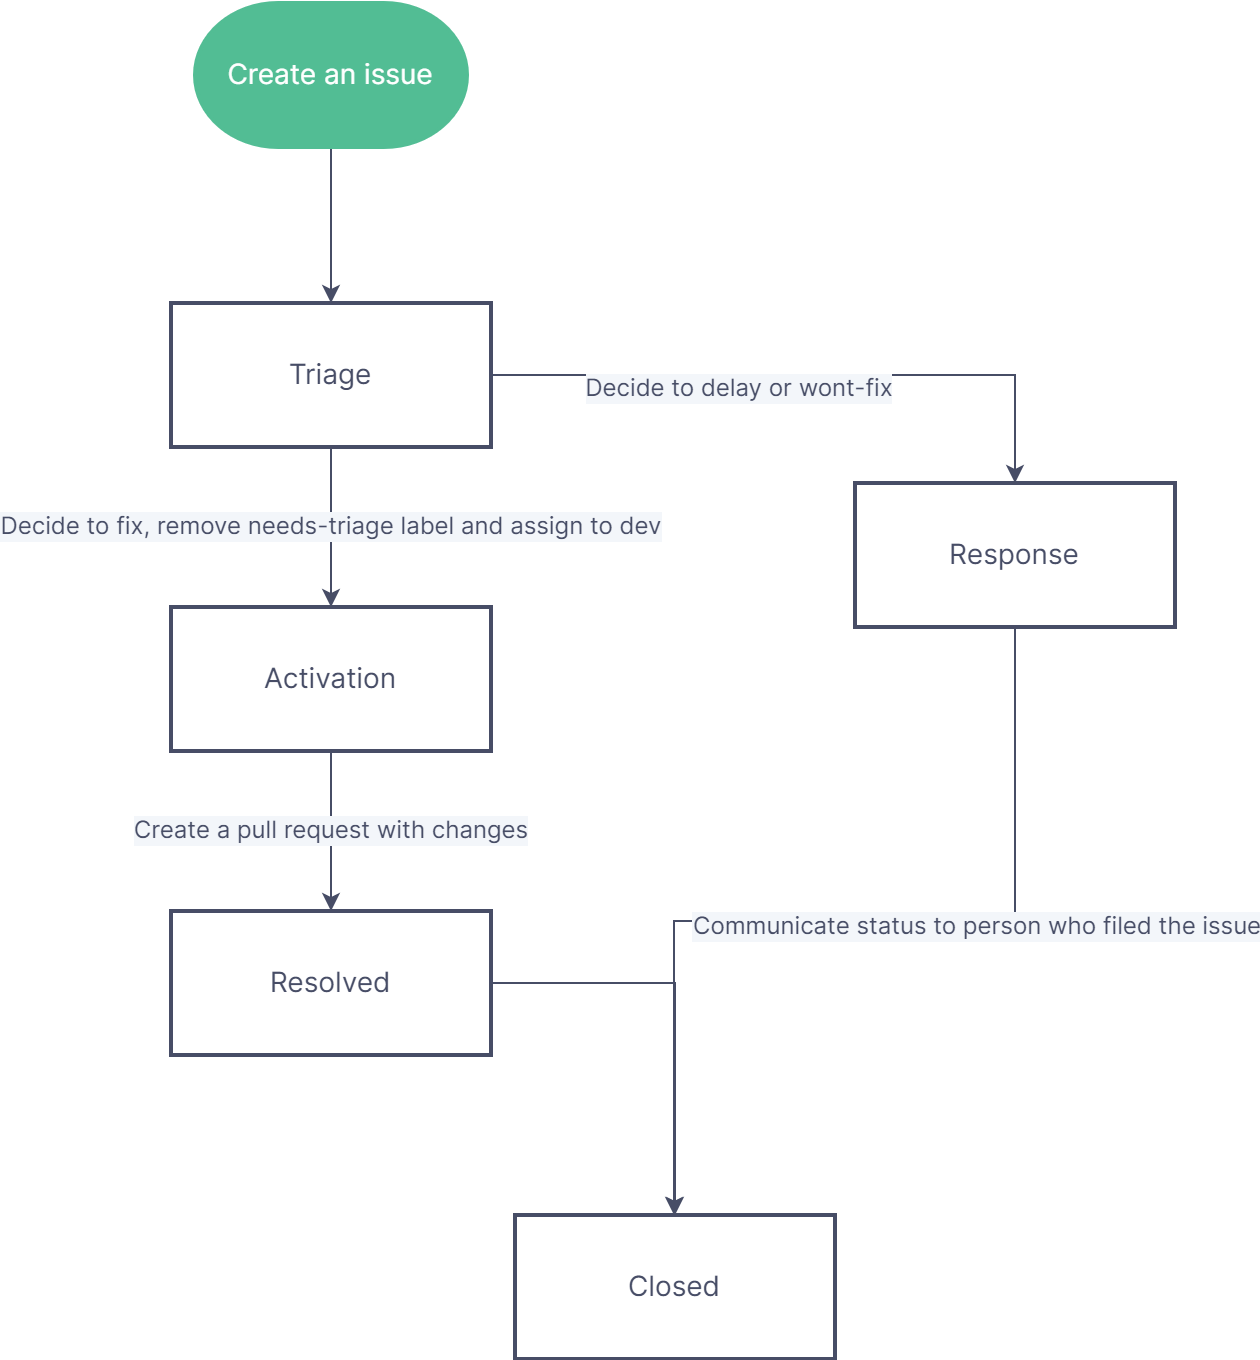
\includegraphics[width=0.75\linewidth]{New Flowchart} \caption{Flow chart that describes above process visually, e.g. how an issue moves from creation, to activation, to response or resolution, and is finally closed.}\label{fig:flowchart}
\end{figure}

\hypertarget{pull-requests}{%
\section{Pull Requests}\label{pull-requests}}

Pull requests are used to identify changes pushed to development branches. Open pull requests allow the FIMS Development Team to discuss and review the changes, as well as add follow-up commits before merging to the main branch. As noted above in the branching stratgegy section, branches, commits, and pull requests should be kept small to enable rapid review and reduce the chance of merge conflicts. Any pull requests for the FIMS Project must be fully tested and reviewed before being merged into the main branch.
Use the \href{https://github.com/NOAA-FIMS/FIMS/blob/main/.github/PULL_REQUEST_TEMPLATE/pull_request_template.md}{pull request template} to create pull requests. Pull requests without this template attached will not be approved.

\hypertarget{code-review}{%
\section{Code Review}\label{code-review}}

Code review ensures health and continuous improvement of the FIMS codebase, while simultaneously helping FIMS developers become familiar with the codebase and ensure there is a diverse team of knolwedgable collaborators to support the continued development and maintenance of FIMS. CI/CD requires rapid review of all new/modified code, so processes must be in place to support this pace. FIMS code review will utilize tools available via \href{https://github.com/features/code-review}{GitHub}, which allows reviewers to analyze code changes, provide inline comments, and view change histories.

\hypertarget{assigning-reviewers}{%
\subsection{Assigning Reviewers}\label{assigning-reviewers}}

Reviewers for the FIMS Project may be assigned in two different ways:

\begin{enumerate}
\def\labelenumi{\arabic{enumi}.}
\tightlist
\item
  A specific member of the FIMS Development Team is requested to review a pull request, based on their specific expertise.
\item
  Code review assignments are automatically assigned using the \href{https://docs.github.com/en/organizations/organizing-members-into-teams/managing-code-review-settings-for-your-team}{GitHub load balance routing algorithm}; this approach tries to ensure that each team member reviews an equal number of pull request in any 30 day period.
\end{enumerate}

Team members should keep their status in Github current (see \href{https://docs.github.com/en/account-and-profile/setting-up-and-managing-your-github-profile/customizing-your-profile/personalizing-your-profile\#setting-a-status}{``Setting a status''} for more information). Reviews will not be auto-assigned to ``Busy'' team members.

If a review has been assigned to you and you don't feel like you have the expertise to address it properly, please respond directly to the code owner immediately so a different reviewer can be found promptly.

\hypertarget{automated-testing}{%
\subsection{Automated Testing}\label{automated-testing}}

Automated testing provides an initial layer of quality assurance and lets reviewers know that the code meets certain standards. For more on FIMS testing, see \href{https://noaa-fims.github.io/collaborative_workflow/test-case-template.html}{Chapter 6}.

\hypertarget{review-checklist}{%
\subsection{Review Checklist}\label{review-checklist}}

While automated testing can assure the code structure and logic pass quality checks, human reviewers are required to evaluate things like functionality, readability, etc. Reviewers should evaluate the code critically and provide comment/feedback on the following items:

\textbf{Readability}

\begin{itemize}
\tightlist
\item
  Is the code easy to understand?
\item
  Are there any parts of the code that are confusing?
\item
  Is the data flow easy to understand?
\item
  Is there any code commented out?
\item
  Does the code include any unclear names?
\item
  Does the code include any errors, repeats, or incomplete sections?
\end{itemize}

\textbf{Functionality}

\begin{itemize}
\tightlist
\item
  Does the code function as it is expected to?
\item
  How will the change impact other parts of the system?
\item
  Are there any unhandled edge cases?
\item
  Are there other code improvements possible?
\end{itemize}

\textbf{Design}

\begin{itemize}
\tightlist
\item
  Are files organized intuitively?
\item
  Are components divided up in a sensible way?
\item
  Does the review include too many changes? Would the code change better be broken into more focused parts?
\item
  Will the change be easy to maintain?
\item
  Does the code follow object-oriented design principles?
\item
  Is the code in the proper location?
\end{itemize}

\textbf{Security}

\begin{itemize}
\tightlist
\item
  Does using this code open the software to possible security violations or vulnerabilities?
\item
  Is the correct encryption used?
\end{itemize}

\textbf{Performance}

\begin{itemize}
\tightlist
\item
  Are there ways to improve on the code's performance?
\item
  Is there any complex logic that could be simplified?
\item
  Could any of the code be replaced with built-in functions?
\item
  Will this change have any impacts on system performance?
\item
  Is there any debugging code that could be removed?
\item
  Are there any optimizations that could be removed and still maintain system performance?
\end{itemize}

\textbf{Documentation}

\begin{itemize}
\tightlist
\item
  Are there comments available to explain the code?
\item
  Is the README file complete and current? Does it adequately describe the project/changes?
\end{itemize}

\textbf{Testing}

\begin{itemize}
\tightlist
\item
  Is the code testable?
\item
  Is the automated testing adequate?
\item
  Have dependencies been appropriately tested?
\item
  Does automated testing cover the code exchange adequately?
\item
  Could the test structure be improved?
\end{itemize}

\hypertarget{review-good-practices}{%
\subsection{Review Good Practices}\label{review-good-practices}}

Good reviews require good review habits. Try to follow these suggestions:

\begin{itemize}
\tightlist
\item
  Review in short sessions (\textless{} 60 minutes) to maintain focus and attention to detail
\item
  Don't try to review more than 400 lines of code in a single session
\item
  Provide constructive and supportive feedback
\item
  Ask open-ended questions and offer alternatives or possible workarounds
\item
  Avoid strong/opinionated statements
\item
  Applaud good solutions
\item
  Don't say ``you''
\item
  Be clear about which questions/comments are non-blocking or unimportant; likewise, be explicit when approving a change or requesting follow-up
\item
  Aim to minimize the number of nitpicks (if there are a lot, suggest a team-level resolution)
\item
  Use the \href{https://noaa-fims.github.io/collaborative_workflow/style-guide.html}{FIMS Style Guide} to settle any style arguments
\end{itemize}

\hypertarget{commit-messages}{%
\section{Commit Messages}\label{commit-messages}}

FIMS Project contributors should provide clear, descriptive commit messages to communicate to collaborators details about changes that have occurred and improve team efficiency. Good commit messages follow the following practices:

\begin{itemize}
\item
  Include a short summary of the change for the subject/title (\textless50 characters)
\item
  Include a blank line in between the `subject' and `body'
\item
  Specify the type of commit:

\begin{verbatim}
    * fix: bug fix
    * feat: new feature
    * test: testing
    * docs: documentation
    * chore: regular code maintenance (e.g. updating dependencies)
    * refactor: refactoring codebase
    * style: changes that do not affect the meaning of the code; instead address code styling/formmatting
    * perf: performance improvements
    * revert: reverts a previous commit
    * build: changes that affect the build system
\end{verbatim}
\item
  If the commit addresses an issue, indicate the issue\# in the title
\item
  Provide a brief explanatory description of the change, addressing what and why was changed
\item
  Wrap to \textasciitilde72 characters
\item
  Write in the imperative (e.g.~``Fix bug'', not ``Fixed bug'')
\item
  If necessary, separate paragraphs by blank lines
\item
  Utilize \texttt{BREAKING\ CHANGE:\ \textless{}description\textgreater{}} to provide expanation or further context about the issue being addressed.
\item
  If the commit closes an issue, include a footer to note that (i.e.~``Closes \#19'')
\end{itemize}

\hypertarget{software-user-guide}{%
\chapter{Software user guide}\label{software-user-guide}}

This section describes how to install and run the model.

\hypertarget{installing-the-package-from-github}{%
\section{Installing the package from Github}\label{installing-the-package-from-github}}

\hypertarget{windows-users}{%
\subsection{Windows users}\label{windows-users}}

Before you install the \texttt{FIMS} package, you will need to install the Rtools executable corresponding to your \texttt{R} version as well as the \texttt{TMB} package and its dependencies. \texttt{FIMS} has only been developed and tested on \texttt{R} version 4.+, and so in order to install the package you will need to ensure you are using \texttt{R} version 4.+ and an RStudio version that is at least 1.2.5042. Instructions on how to install \texttt{Rtools} are \href{https://cran.r-project.org/bin/windows/Rtools/rtools40.html}{here}. Instructions on how to install \texttt{TMB} are \href{https://github.com/kaskr/adcomp/wiki/Download}{here}. Please ensure you have tested your \texttt{TMB} setup before moving on to install FIMS.

\hypertarget{mac-users}{%
\subsection{Mac users}\label{mac-users}}

\hypertarget{linux-users}{%
\subsection{Linux users}\label{linux-users}}

\hypertarget{installing-from-r}{%
\section{\texorpdfstring{Installing from \texttt{R}}{Installing from R}}\label{installing-from-r}}

\begin{Shaded}
\begin{Highlighting}[]
\NormalTok{remotes}\SpecialCharTok{::}\FunctionTok{install\_github}\NormalTok{(}\StringTok{"NOAA{-}FIMS/FIMS"}\NormalTok{)}
\FunctionTok{library}\NormalTok{(FIMS)}
\end{Highlighting}
\end{Shaded}

\hypertarget{specifying-and-compiling-the-model}{%
\section{Specifying and compiling the model}\label{specifying-and-compiling-the-model}}

You can add components to the model using S4 classes.

\begin{Shaded}
\begin{Highlighting}[]
\CommentTok{\#TODO: add script to populate the model}
\end{Highlighting}
\end{Shaded}

\hypertarget{extracting-model-output}{%
\section{Extracting model output}\label{extracting-model-output}}

Here is how you get the model output.

\begin{Shaded}
\begin{Highlighting}[]
\CommentTok{\#Todo add code for how to extract model output}
\end{Highlighting}
\end{Shaded}

\hypertarget{model-specification}{%
\chapter{Model specification}\label{model-specification}}

This section describes the implementation of the modules in FIMS in milestone 1. For the first milestone, we must implement enough complexity to adequately test a very standard population model. For this reason, we implement the minimum structure that can run the model described in \href{}{Li et al.~2020}.

\hypertarget{model-variables-and-bounds}{%
\section{Model variables and bounds}\label{model-variables-and-bounds}}

\hypertarget{inherited-functors-from-tmb}{%
\section{\texorpdfstring{Inherited functors from \texttt{TMB}}{Inherited functors from TMB}}\label{inherited-functors-from-tmb}}

\hypertarget{atomic-functions}{%
\subsection{Atomic functions}\label{atomic-functions}}

Wherever possible, \texttt{FIMS} should not reinvent atomic functions with extant definitions in \texttt{TMB}. If there is a need for a new atomic function the development team can add it to \texttt{TMB} using the \texttt{TMB\_ATOMIC\_VECTOR\_FUNCTION()} macro following the instructions \href{https://kaskr.github.io/adcomp/_book/AtomicFunctions.html\#example-adding-new-primitive-function-with-known-derivatives}{here}.

\hypertarget{statistical-distributions}{%
\subsection{Statistical distributions}\label{statistical-distributions}}

All of the statistical distributions needed for the first milestone of \texttt{FIMS} are implemented in \texttt{TMB} and need not be replicated.
Code can be found \href{http://kaskr.github.io/adcomp/group__R__style__distribution.html}{here}.
\textbar Distribution \textbar{} Name\textbar{}
\textbar{} ------------\textbar---------\textbar{}
\textbar Normal \textbar{} \href{http://kaskr.github.io/adcomp/dnorm_8hpp.html}{dnorm}\textbar{}
\textbar Multinomial \textbar{} \href{http://kaskr.github.io/adcomp/group__R__style__distribution.html\#gafd0ae6b53840267138bb9250115fbe8b}{dmultinom}\\

\hypertarget{beverton-holt-expected-recruitment-function}{%
\section{Beverton-Holt expected recruitment function}\label{beverton-holt-expected-recruitment-function}}

For parity with existing stock assessment models, the first recruitment option in FIMS is a Beverton-Holt {[}cite{]} parameterized with R0 and h.

\[R_t  =\frac{0.8R_0hS_{t-1}}{0.2R_0\phi_0(1-h) + S_{t-1}(h-0.2)}\]
Where \(R_t\) and \(S_t\) are mean recruitment and spawning biomass in time \(t\), \(h\) is Mace-Doonan steepness, and \(\phi_0\) are the unfished spawning biomass per recruit. The initial FIMS model will implement a static spawning biomass-per-recruit function, with the ability to overload the method in the future to allow for time-variation in mortality, maturity, and weight-at-age over time to account for changes in spawning biomass per recruit. Deviations are assumed to be lognormally distributed such that realized recruitment is the product of mean recruitment and the exponentiated recruitment deviation.
\[R_t = R_t\mathrm{exp}(r_{dev,t}-R^2/2),   r_{dev,t} \sim N(0,R^2)\]

However, true \(r_{dev,t}\) values are not known, so when using estimated recruitment deviations \(\hat{r_{dev,t}}\) the following equation is applied to calculate mean unbiased recruitment \(R*_t\) using a bias adjustment factor \(b_y=\frac{E[SD(ry)]^2}{\sigma_R^2}\) (Methot and Taylor, 2011).
\[R^*_t=R_t\mathrm{exp}(\hat{r_{dev,t}}-b_y\frac{\sigma_R^2}{2})\]
The recruitment function should take as input the \(R\) , \(S\) values, the \(h\), \(ln(R_0)\), and R parameters and \(\phi_0\) and return mean and realized recruitment.

\hypertarget{logistic-function-with-extensions}{%
\section{Logistic function with extensions}\label{logistic-function-with-extensions}}

\[x_i=\frac{1}{1+\mathrm{exp}(-ln(19)(i-\nu_1)/\nu_2)}\]

Where \(x_i\) is the quantity of interest (proportion mature, selected, etc.), \(i\) is the index (can be age or size or any other quantity),
\(\nu_1\) is the index of 50\% mature and \(\nu_2\) is the difference in the index at 50\% and the index at 95\% (\(\nu_2 = \mathrm{ln}(19)/s\) where
\(s\) is the slope parameter from an alternative parameterization). Logistic functions for maturity and selectivity should inherit and extend
upon the base logistic function implementation.

\hypertarget{catch-and-fishing-mortality}{%
\section{Catch and fishing mortality}\label{catch-and-fishing-mortality}}

The Baranov catch equation relates catch to instantaneous fishing and natural mortality.

\[ C_{f,a,t}=\frac{F_{f,a,t}}{F_{f,a,t}+M}(1-\mathrm{exp}(-(F_{f,a,t}+M)))N_{a,t}\]

Where \(C_{f,a,t}\) is the catch at age \(a\) at time \(t\) for fleet \(f\), \(F\) is instantaneous fishing mortality,
\(M\) is assumed constant over ages and time in the minimum viable assessment model, \(N_a,t\) is the number of
age \(a\) fish at time \(t\).

\[F_{a,t}=\sum_{a=0}^A s_{a,f,t}F\]

\(s_a,f\) is selectivity at age \(a\) for fleet \(f\). Selectivity-at-age is constant over time.

Catch is in metric tons and survey is in number, so calculating catch weight (\(CW_t\)) is done as follows:
\[ CW_t=\sum_{a=0}^A C_{a,t}w_a \]

Survey numbers are calculated as follows

\[I_t=q\sum_{a=0}^AN_{a,t}\]
Where \(I_t\) is the survey index and \(q_t\) is survey catchability at time \(t\).

\hypertarget{modeling-loops}{%
\section{Modeling loops}\label{modeling-loops}}

This tier associates the expected values for each population section associated with a data source to that data source using a likelihood function. These likelihood functions are then combined into an objective function that is passed to TMB.

The population loop will be initialized at a user-specified age, time increment, and seasonal structure, rather than assuming ages, years, or seasons follow any pre-defined structure. Population categories will be described flexibly, such that subpopulations such as unique sexes, stocks, species, or areas can be handled identically to reduce duplication. Each subpopulation will have a unique set of attributes assigned to it, such that each subpopulation can share or have a different functional process (e.g.~recruitment function, size-at-age) than a different category.

Spawning time and recruitment time are user-specified and can occur more than once per year. For the purposes of replicating model comparison project outputs, in milestone 1, all processes including spawning and recruitment occur January 1, but these should be specified via the \texttt{spawn\_time} and \texttt{recruit\_time} inputs into FIMS to allow for future flexibility. Spawning and recruitment timing can be input as a scalar or vector to account for multiple options.

Within the population loop, matrices denoting population properties at different partitions (age, season, sex) are translated into a single, dimension-folded index. A lookup table is computed at model start so that the dimension-folded index can be mapped to its corresponding population partition or time partition (e.g.~population(sex, area, age, species, time, \ldots)) so the programmer can understand what is happening. The model steps through each specified timestep to match the data to expected values, and population processes occur in the closest specified timestep to the user-input process timing (e.g.~recruitment) across a small timestep that is a predefined constant.

\hypertarget{expected-numbers-and-quantities}{%
\section{Expected numbers and quantities}\label{expected-numbers-and-quantities}}

The expected values are calculated as follows in the population.hpp file:
\[ B_t=\sum_{a=0}^AN_{a,t}w_a\]
where \(B_t\) is total biomass in time \(t\), \(N\) is total numbers, \(w_a\) is weight-at-age \(a\) in kilograms.

\[N_t=\sum_{a=0}^AN_{a,t}\]
where \(N_t\) is the total number of fish in time \(t\).

\hypertarget{initial-values}{%
\section{Initial values}\label{initial-values}}

\hypertarget{initial-n}{%
\subsection{Initial N}\label{initial-n}}

\hypertarget{initial-f}{%
\subsection{Initial F}\label{initial-f}}

\hypertarget{likelihood-calculations}{%
\section{Likelihood calculations}\label{likelihood-calculations}}

Age composition likelihood links proportions at age from data to model using a multinomial likelihood function. The multinomial and lognormal distributions, including atomic functions are provided within \texttt{TMB}.

Survey index likelihood links estimated CPUE to input data CPUE in biomass using a lognormal distribution. (model.hpp)

Catch index likelihood links estimated catch to input data catch in biomass using a lognormal distribution. (model.hpp)

Age composition likelihoods link catch-at-age to expected catch-at-age using a multinomial distribution.

\hypertarget{hpp-template-for-c-modules}{%
\chapter{.hpp template for C++ modules}\label{hpp-template-for-c-modules}}

In this section we will describe how to structure a new .hpp file in FIMS.

\begin{Shaded}
\begin{Highlighting}[]
\CommentTok{//  tmplate.hpp}
\CommentTok{//  Fisheries Integrated Modeling System (FIMS)}

\CommentTok{//define the header gaurd}
\PreprocessorTok{\#ifndef template\_hpp }
\PreprocessorTok{\#define template\_hpp}

\CommentTok{//inherit from model\_base}
\PreprocessorTok{\#include }\ImportTok{"../common.hpp"}\PreprocessorTok{ }
\PreprocessorTok{\#include }\ImportTok{\textless{}iostream\textgreater{}}

\CommentTok{/**}
\CommentTok{ * In this example, we utilize the concept of inheritence and }
\CommentTok{ * polymorphism (https://www.geeksforgeeks.org/polymorphism{-}in{-}c/). All}
\CommentTok{ * classes inherit from model\_base. Name1 and Name2 inherit from NameBase.}
\CommentTok{ * Classes Name1 and Name2 must implement they\textquotesingle{}re own version of }
\CommentTok{ * "virtual T evaluate(const T\& t)", which will have unique logic. }
\CommentTok{ */}


\CommentTok{/*}
\CommentTok{ * fims namespace}
\CommentTok{ */}
\NormalTok{namespace fims}\OperatorTok{\{}

\CommentTok{/**}
\CommentTok{ * NameBase class. Inherits from model\_base.}
\CommentTok{ */}
\NormalTok{template }\OperatorTok{\textless{}}\NormalTok{class T}\OperatorTok{\textgreater{}}
\NormalTok{class NameBase}\OperatorTok{:}\NormalTok{ public model\_base}\OperatorTok{\textless{}}\NormalTok{T}\OperatorTok{\textgreater{}\{} \CommentTok{//note that model\_base gets template parameter T.}
\NormalTok{protected}\OperatorTok{:}

\NormalTok{public}\OperatorTok{:}
\NormalTok{  virtual T Evaluate}\OperatorTok{(}\DataTypeTok{const}\NormalTok{ T}\OperatorTok{\&}\NormalTok{ t}\OperatorTok{)=}\DecValTok{0}\OperatorTok{;} \CommentTok{//"= 0;" means this must be implemented in child.}
\OperatorTok{\};}
  
\CommentTok{/* }
\CommentTok{* Template class inherits from  NameBase}
\CommentTok{*/}
\NormalTok{template }\OperatorTok{\textless{}}\NormalTok{class T}\OperatorTok{\textgreater{}}
\NormalTok{class Name1}\OperatorTok{:}\NormalTok{ public NameBase}\OperatorTok{\textless{}}\NormalTok{T}\OperatorTok{\textgreater{}\{}

\NormalTok{public}\OperatorTok{:}
 
    
  \CommentTok{/*}
\CommentTok{   *Default constructor}
\CommentTok{   *Initialize any memory here.}
\CommentTok{   */}
\NormalTok{  Name1}\OperatorTok{()\{}
  \OperatorTok{\}}
  
 
  \CommentTok{/**}
\CommentTok{   * Destructor; this method destructs Name1 object.}
\CommentTok{   * Delete any allocated memory here.}
\CommentTok{   */}
  \OperatorTok{\textasciitilde{}}\NormalTok{ Name1}\OperatorTok{()\{}
\NormalTok{    std}\OperatorTok{::}\NormalTok{cout }\OperatorTok{\textless{}\textless{}}\StringTok{"I just deleted Name1 object"} \OperatorTok{\textless{}\textless{}}\NormalTok{ std}\OperatorTok{::}\NormalTok{endl}\OperatorTok{;}
  \OperatorTok{\}}
  
   \CommentTok{/**}
\CommentTok{    * Note: this function must have the same signature as evaluate in NameBase.}
\CommentTok{    * Overloaded virtual function. This is polymorphism, meaning the }
\CommentTok{    * signature has the same appearance, but the function itself has unique logic.}
\CommentTok{    * }
\CommentTok{    * }\AnnotationTok{@param}\CommentTok{ t}
\CommentTok{    * }\AnnotationTok{@return}\CommentTok{ t+1}
\CommentTok{    */}
\NormalTok{   virtual T Evaluate}\OperatorTok{(}\DataTypeTok{const}\NormalTok{ T}\OperatorTok{\&}\NormalTok{ t}\OperatorTok{)} \OperatorTok{\{}
\NormalTok{     std}\OperatorTok{::}\NormalTok{cout}\OperatorTok{\textless{}\textless{}}\StringTok{"evaluate in Name1 received "}\OperatorTok{\textless{}\textless{}}\NormalTok{t}\OperatorTok{\textless{}\textless{}}
     \StringTok{"as a method parameter, returning "}\OperatorTok{\textless{}\textless{}(}\NormalTok{t}\OperatorTok{+}\DecValTok{1}\OperatorTok{)\textless{}\textless{}}\NormalTok{std}\OperatorTok{::}\NormalTok{endl}\OperatorTok{;}
     \ControlFlowTok{return}\NormalTok{ t}\OperatorTok{+}\DecValTok{1}\OperatorTok{;} \CommentTok{//unique logic for Name1 class}
   \OperatorTok{\}}

\OperatorTok{\};}

  \CommentTok{/* }
\CommentTok{* Template class inherits from  NameBase}
\CommentTok{*/}
\NormalTok{template }\OperatorTok{\textless{}}\NormalTok{class T}\OperatorTok{\textgreater{}}
\NormalTok{class Name2}\OperatorTok{:}\NormalTok{ public NameBase}\OperatorTok{\textless{}}\NormalTok{T}\OperatorTok{\textgreater{}\{}

\NormalTok{public}\OperatorTok{:}
 
    
  \CommentTok{/*}
\CommentTok{   *Default constructor.}
\CommentTok{   *Initialize any memory here.}
\CommentTok{   */}
\NormalTok{  Name2}\OperatorTok{()\{}
  \OperatorTok{\}}
  
 
  \CommentTok{/**}
\CommentTok{   * Destructor; this method destructs the Name2 object.}
\CommentTok{   * Delete any allocated memory here.}
\CommentTok{   */}
  \OperatorTok{\textasciitilde{}}\NormalTok{ Name2}\OperatorTok{()\{}
\NormalTok{    std}\OperatorTok{::}\NormalTok{cout }\OperatorTok{\textless{}\textless{}}\StringTok{"I just deleted Name2 object"} \OperatorTok{\textless{}\textless{}}\NormalTok{ std}\OperatorTok{::}\NormalTok{endl}\OperatorTok{;}
  \OperatorTok{\}}
  
   \CommentTok{/**}
\CommentTok{    * Note: this function must have the same signature as evaluate in NameBase.}
\CommentTok{    * Overloaded virtual function. This is polymorphism, meaning the }
\CommentTok{    * signature has the same appearance, but the function itself has unique logic.}
\CommentTok{    * }
\CommentTok{    * }\AnnotationTok{@param}\CommentTok{ t}
\CommentTok{    * }\AnnotationTok{@return}\CommentTok{ t\^{}2}
\CommentTok{    */}
\NormalTok{   virtual T Evaluate}\OperatorTok{(}\DataTypeTok{const}\NormalTok{ T}\OperatorTok{\&}\NormalTok{ t}\OperatorTok{)} \OperatorTok{\{}
\NormalTok{     std}\OperatorTok{::}\NormalTok{cout}\OperatorTok{\textless{}\textless{}}\StringTok{"evaluate in Name2 received "}\OperatorTok{\textless{}\textless{}}\NormalTok{t}\OperatorTok{\textless{}\textless{}}
     \StringTok{"as a method parameter, returning "}\OperatorTok{\textless{}\textless{}(}\NormalTok{t}\OperatorTok{*}\NormalTok{t}\OperatorTok{)\textless{}\textless{}}\NormalTok{std}\OperatorTok{::}\NormalTok{endl}\OperatorTok{;}
     \ControlFlowTok{return}\NormalTok{ t}\OperatorTok{*}\NormalTok{t}\OperatorTok{;} \CommentTok{//unique logic for Name2 class}
   \OperatorTok{\}}

\OperatorTok{\};}
  
\CommentTok{/**}
\CommentTok{ * Add additional implementations below.}
\CommentTok{ */}
  



\OperatorTok{\}} \CommentTok{//end namespace}

\CommentTok{/**}
\CommentTok{ *Example usage:}
\CommentTok{ *}
\CommentTok{ * void main(int argc, char** argv)\{}
\CommentTok{ *    NameBase}\KeywordTok{\textless{}double\textgreater{}}\CommentTok{* name = NULL; //pointer to a NameBase object}
\CommentTok{ *    Name1}\KeywordTok{\textless{}double\textgreater{}}\CommentTok{ n1; //inherits from NameBase}
\CommentTok{ *    Name2}\KeywordTok{\textless{}double\textgreater{}}\CommentTok{ n2; //inherits from NameBase}
\CommentTok{ *}
\CommentTok{ *    name = \&n1; //name now points to n1}
\CommentTok{ *    name{-}\textgreater{}Evalute(2.0); //unique logic for n1}
\CommentTok{ *}
\CommentTok{ *    name = \&n2; //name now points to n2}
\CommentTok{ *    name{-}\textgreater{}Evalute(2.0); //unique logic for n2}
\CommentTok{ * \}}
\CommentTok{ *}
\CommentTok{ * Output:}
\CommentTok{ * evaluate in Name1 received 2 as a method parameter, returning 3}
\CommentTok{ * evaluate in Name2 received 2 as a method parameter, returning 4}
\CommentTok{ *}
\CommentTok{ */}



\PreprocessorTok{\#endif }\CommentTok{/*template\_hpp */}
\end{Highlighting}
\end{Shaded}

\hypertarget{test-case-template}{%
\chapter{Test case template}\label{test-case-template}}

In this section we will describe how to write a test case for your FIMS code.

\hypertarget{introduction}{%
\section{Introduction}\label{introduction}}

FIMS testing framework will include different types of testing to make sure that changes to FIMS code are working as expected. The unit and functional tests will be developed during the initial development stage when writing individual functions or modules. After completing development of multiple modules, integration testing will be developed to verify that different modules work well together. Checks will be added in the software to catch user input errors when conducting run-time testing. Regression testing and platform compatibility testing will be executed before pre-releasing FIMS. Beta-testing will be used to gather feedback from users (i.e., members of FIMS implementation team and other users) during the pre-release stage. After releasing the first version of FIMS, the development team will go back to the beginning of the testing cycle and write unit tests when a new feature needs to be implemented. One-off testing will be used for testing new features and fixing user-reported bugs when maintaining FIMS. More details of each type of test can be found in the Glossary section.

FIMS will use GoogleTest to build a C++ unit testing framework and R testthat to build an R testing framework. FIMS will use Google Benchmark to measure the real time and CPU time used for running the produced binaries.

\hypertarget{c-unit-testing-and-benchmarking}{%
\section{C++ unit testing and benchmarking}\label{c-unit-testing-and-benchmarking}}

\hypertarget{requirements}{%
\subsection{Requirements}\label{requirements}}

To use GoogleTest, you will need:

\begin{itemize}
\item
  A compatible operating system (e.g.~Windows, masOS, or Linux).
\item
  A C++ compiler that supports at least C++ 11 standard or newer (e.g.~gcc 5.0+, clang 5.0+, or MSVC 2015+). For macOS users, Xcode 9.3+ provides clang 5.0.
\item
  A build system for building the testing project. \href{https://cmake.org/}{\underline{CMake}} and a compatible build tool such as \href{https://ninja-build.org/}{\underline{Ninja}} are approved softwares by NMFS HQ.
\end{itemize}

\hypertarget{quickstart-for-windows-user}{%
\subsection{Quickstart for Windows user}\label{quickstart-for-windows-user}}

\begin{itemize}
\item
  Download \href{https://github.com/Kitware/CMake/releases}{\underline{CMake 3.22.1 (cmake-3.22.1-windows-x86\_64.zip)}} and put the file folder to \texttt{Documents\textbackslash{}Apps} or other preferred folder.
\item
  Download \href{https://github.com/ninja-build/ninja/releases}{\underline{ninja v1.10.2 (ninja-win.zip)}} and put the application to \texttt{Documents\textbackslash{}Apps} or other preferred folder.
\item
  Search \texttt{Edit\ environment\ variables\ for\ your\ account} and open the \texttt{Environment\ Variables} window.
\item
  Click \texttt{Edit...} under the \texttt{User\ variables\ for\ firstname.lastname} section.
\item
  Click \texttt{New}, add path to \texttt{cmake-3.22.1-windows-x86\_64\textbackslash{}bin}, add click \texttt{OK}.
\item
  Click \texttt{New}, add path to \texttt{Documents\textbackslash{}Apps}, add click \texttt{OK}.
\item
  Open your Command Prompt and type \texttt{cmake}. If you see details of usage, you install the build system successfully.
\item
  See \href{https://cmake.org/install}{\underline{CMake installation instructions}} for installing CMake on other platforms.
\end{itemize}

\hypertarget{set-up-fims-testing-project}{%
\subsection{Set up FIMS testing project}\label{set-up-fims-testing-project}}

\begin{itemize}
\tightlist
\item
  Go to the FIMS C++ tests folder and create a \texttt{CMakeLists.txt} file. Declare a dependency on GoogleTest with following contents:
\end{itemize}

\begin{Shaded}
\begin{Highlighting}[]
\KeywordTok{cmake\_minimum\_required}\NormalTok{(}\OtherTok{VERSION} \DataTypeTok{3.14}\NormalTok{)}
\KeywordTok{project}\NormalTok{(FIMS\_project)}

\CommentTok{\# GoogleTest requires at least C++11}
\KeywordTok{set}\NormalTok{(}\DecValTok{CMAKE\_CXX\_STANDARD}\NormalTok{ 11)}

\KeywordTok{include}\NormalTok{(FetchContent)}
\FunctionTok{FetchContent\_Declare}\NormalTok{(}
\NormalTok{  googletest}
\NormalTok{  URL https://github.com/google/googletest/archive/refs/tags/release{-}}\DataTypeTok{1.11.0}\NormalTok{.zip}
\NormalTok{)}

\CommentTok{\# For Windows: Prevent overriding the parent project\textquotesingle{}s compiler/linker settings}
\KeywordTok{set}\NormalTok{(gtest\_force\_shared\_crt }\OtherTok{ON} \OtherTok{CACHE} \OtherTok{BOOL} \StringTok{""} \OtherTok{FORCE}\NormalTok{)}
\FunctionTok{FetchContent\_MakeAvailable}\NormalTok{(googletest)}
\end{Highlighting}
\end{Shaded}

\begin{itemize}
\tightlist
\item
  If a \texttt{CMakeLists.txt} file already exists in the tests folder, you can start creating a unit test and add it to the \texttt{CMakeLists.txt}.
\end{itemize}

\hypertarget{unit-test-template}{%
\subsection{Unit test template}\label{unit-test-template}}

\begin{Shaded}
\begin{Highlighting}[]
\PreprocessorTok{\#include }\ImportTok{"gtest/gtest.h"}
\PreprocessorTok{\#include }\ImportTok{"../src/code.hpp"}

\CommentTok{// \# R code that generates true values for the test}

\NormalTok{namespace }\OperatorTok{\{}

  \CommentTok{// Description of Test 1 }
\NormalTok{  TEST}\OperatorTok{(}\NormalTok{TestSuiteName}\OperatorTok{,}\NormalTok{ Test1Name}\OperatorTok{)} \OperatorTok{\{}
    
    \OperatorTok{...}\NormalTok{ test body }\OperatorTok{...} 
    
  \OperatorTok{\}}
  
  \CommentTok{// Description of Test 2}
\NormalTok{  TEST}\OperatorTok{(}\NormalTok{TestSuiteName}\OperatorTok{,}\NormalTok{ Test2Name}\OperatorTok{)} \OperatorTok{\{}
    
    \OperatorTok{...}\NormalTok{ test body }\OperatorTok{...}
    
  \OperatorTok{\}}
  
\OperatorTok{\}}
\end{Highlighting}
\end{Shaded}

\hypertarget{unit-test-example}{%
\subsection{Unit test example}\label{unit-test-example}}

Let's create dlognorm.hpp that has a simple function:

\begin{Shaded}
\begin{Highlighting}[]
\PreprocessorTok{\#include }\ImportTok{\textless{}cmath\textgreater{}}

\NormalTok{template}\OperatorTok{\textless{}}\NormalTok{class Type}\OperatorTok{\textgreater{}}
\NormalTok{Type dlognorm}\OperatorTok{(}\NormalTok{Type x}\OperatorTok{,}\NormalTok{ Type meanlog}\OperatorTok{,}\NormalTok{ Type sdlog}\OperatorTok{)\{}
\NormalTok{  Type resid }\OperatorTok{=} \OperatorTok{(}\NormalTok{log}\OperatorTok{(}\NormalTok{x}\OperatorTok{){-}}\NormalTok{meanlog}\OperatorTok{)/}\NormalTok{sdlog}\OperatorTok{;}
\NormalTok{  Type logres }\OperatorTok{=} \OperatorTok{{-}}\NormalTok{log}\OperatorTok{(}\NormalTok{sqrt}\OperatorTok{(}\DecValTok{2}\OperatorTok{*}\NormalTok{M\_PI}\OperatorTok{))} \OperatorTok{{-}}\NormalTok{ log}\OperatorTok{(}\NormalTok{sdlog}\OperatorTok{)} \OperatorTok{{-}}\NormalTok{ Type}\OperatorTok{(}\FloatTok{0.5}\OperatorTok{)*}\NormalTok{resid}\OperatorTok{*}\NormalTok{resid }\OperatorTok{{-}}\NormalTok{ log}\OperatorTok{(}\NormalTok{x}\OperatorTok{);}
  \ControlFlowTok{return}\NormalTok{ logres}\OperatorTok{;} 
\OperatorTok{\}}
\end{Highlighting}
\end{Shaded}

We can create a test file dlognorm-unit.cpp that has a test suite for this function:

\begin{Shaded}
\begin{Highlighting}[]
\PreprocessorTok{\#include }\ImportTok{"gtest/gtest.h"}
\PreprocessorTok{\#include }\ImportTok{"../src/dlognorm.hpp"}

\CommentTok{// \# R code that generates true values for the test}
\CommentTok{// dlnorm(1.0, 0.0, 1.0, TRUE) = {-}0.9189385}
\CommentTok{// dlnorm(5.0, 10.0, 2.5, TRUE) = {-}9.07679}

\NormalTok{namespace }\OperatorTok{\{}

  \CommentTok{// TestSuiteName: dlognormTest; TestName: DoubleInput and IntInput}
  \CommentTok{// Test dlognorm with double input values}
  
\NormalTok{  TEST}\OperatorTok{(}\NormalTok{dlognormTest}\OperatorTok{,}\NormalTok{ DoubleInput}\OperatorTok{)} \OperatorTok{\{}
    
\NormalTok{    EXPECT\_NEAR}\OperatorTok{(}\NormalTok{ dlognorm}\OperatorTok{(}\FloatTok{1.0}\OperatorTok{,} \FloatTok{0.0}\OperatorTok{,} \FloatTok{1.0}\OperatorTok{)} \OperatorTok{,} \OperatorTok{{-}}\FloatTok{0.9189385} \OperatorTok{,} \FloatTok{0.0001} \OperatorTok{);} 
\NormalTok{    EXPECT\_NEAR}\OperatorTok{(}\NormalTok{ dlognorm}\OperatorTok{(}\FloatTok{5.0}\OperatorTok{,} \FloatTok{10.0}\OperatorTok{,} \FloatTok{2.5}\OperatorTok{)} \OperatorTok{,} \OperatorTok{{-}}\FloatTok{9.07679} \OperatorTok{,} \FloatTok{0.0001} \OperatorTok{);} 
    
  \OperatorTok{\}}
  
  \CommentTok{// Test dlognorm with integer input values}
  
\NormalTok{  TEST}\OperatorTok{(}\NormalTok{dlognormTest}\OperatorTok{,}\NormalTok{ IntInput}\OperatorTok{)} \OperatorTok{\{}
    
\NormalTok{    EXPECT\_NE}\OperatorTok{(}\NormalTok{ dlognorm}\OperatorTok{(}\DecValTok{1}\OperatorTok{,} \DecValTok{0}\OperatorTok{,} \DecValTok{1}\OperatorTok{)} \OperatorTok{,} \OperatorTok{{-}}\FloatTok{0.9189385} \OperatorTok{);}
    
  \OperatorTok{\}}
  
\OperatorTok{\}}
\end{Highlighting}
\end{Shaded}

\texttt{EXPECT\_NEAR(val1,\ val2,\ absolute\_error)} verifies that the difference between \texttt{val1} and \texttt{val2} does not exceed the absolute error bound \texttt{absolute\_error}. \texttt{EXPECT\_NE(val1,\ val2)} verifies that \texttt{val1} is not equal to \texttt{val2}. Please see GoogleTest \href{https://google.github.io/googletest/reference/assertions.html}{assertions reference} for more \texttt{EXPECT\_} macros.

\hypertarget{add-tests-to-cmakelists.txt-and-run-a-binary}{%
\subsection{\texorpdfstring{Add tests to \texttt{CMakeLists.txt} and run a binary}{Add tests to CMakeLists.txt and run a binary}}\label{add-tests-to-cmakelists.txt-and-run-a-binary}}

To build the code, add the following contents to the end of your \texttt{CMakeLists.txt} file:

\begin{Shaded}
\begin{Highlighting}[]
\KeywordTok{enable\_testing}\NormalTok{()}

\KeywordTok{add\_executable}\NormalTok{(}
\NormalTok{  dlognorm\_test}
\NormalTok{  dlognorm{-}unit.cpp}
\NormalTok{)}

\KeywordTok{target\_include\_directories}\NormalTok{(}
\NormalTok{  dlognorm\_test }\OtherTok{PUBLIC}
  \DecValTok{$\{CMAKE\_SOURCE\_DIR\}}\NormalTok{/../}
\NormalTok{)}

\KeywordTok{target\_link\_libraries}\NormalTok{(}
\NormalTok{  dlognorm\_test}
\NormalTok{  gtest\_main}
\NormalTok{)}

\KeywordTok{include}\NormalTok{(GoogleTest)}
\FunctionTok{gtest\_discover\_tests}\NormalTok{(dlognorm\_test)}
\end{Highlighting}
\end{Shaded}

The above configuration enables testing in CMake, declares the C++ test binary you want to build (dlognorm\_test), and links it to GoogleTest (gtest\_main). Now you can build and run your test:

\begin{Shaded}
\begin{Highlighting}[]
\BuiltInTok{cd}\NormalTok{ tests}
\FunctionTok{cmake} \AttributeTok{{-}S}\NormalTok{ . }\AttributeTok{{-}B}\NormalTok{ build }\AttributeTok{{-}G}\NormalTok{ Ninja}
\BuiltInTok{cd}\NormalTok{ build }
\FunctionTok{cmake} \AttributeTok{{-}{-}build}\NormalTok{ .}
\ExtensionTok{ctest}
\end{Highlighting}
\end{Shaded}

The output might look like this:

\begin{Shaded}
\begin{Highlighting}[]
\ExtensionTok{Start}\NormalTok{ 1: dlognormTest.DoubleInput}
\ExtensionTok{1/2}\NormalTok{ Test }\CommentTok{\#1: dlognormTest.DoubleInput .........   Passed    0.11 sec}
\ExtensionTok{Start}\NormalTok{ 2: dlognormTest.IntInput}
\ExtensionTok{2/2}\NormalTok{ Test }\CommentTok{\#2: dlognormTest.IntInput ............   Passed    0.11 sec}

\ExtensionTok{100\%}\NormalTok{ tests passed, 0 tests failed out of 2}

\ExtensionTok{Total}\NormalTok{ Test time }\ErrorTok{(}\ExtensionTok{real}\KeywordTok{)} \ExtensionTok{=}\NormalTok{   0.25 sec}
\end{Highlighting}
\end{Shaded}

Congratulations! You've successfully set up a test project and run a test binary using GoogleTest. Let's use Google Benchmark to measure the real time and CPU time used for running the produced binary.

\hypertarget{benchmark-template}{%
\subsection{Benchmark template}\label{benchmark-template}}

\begin{Shaded}
\begin{Highlighting}[]
\PreprocessorTok{\#include }\ImportTok{"benchmark/benchmark.h"}
\PreprocessorTok{\#include }\ImportTok{"../src/code.hpp"}

\DataTypeTok{void}\NormalTok{ BM\_FunctionName}\OperatorTok{(}\NormalTok{benchmark}\OperatorTok{::}\NormalTok{State}\OperatorTok{\&}\NormalTok{ state}\OperatorTok{)}
\OperatorTok{\{}
  \ControlFlowTok{for} \OperatorTok{(}\DataTypeTok{auto}\NormalTok{ \_ }\OperatorTok{:}\NormalTok{ state}\OperatorTok{)}
    \CommentTok{// This code gets timed}
\NormalTok{    Function}\OperatorTok{()}
\OperatorTok{\}}

\CommentTok{// Register the function as a benchmark}
\NormalTok{BENCHMARK}\OperatorTok{(}\NormalTok{BM\_FunctionName}\OperatorTok{);}
\end{Highlighting}
\end{Shaded}

\hypertarget{benchmark-example}{%
\subsection{Benchmark example}\label{benchmark-example}}

We will continue using the dlognorm.hpp example. We can create a benchmark file dlognorm\_benchmark.cpp and put it in the tests folder:

\begin{Shaded}
\begin{Highlighting}[]
\PreprocessorTok{\#include }\ImportTok{"benchmark/benchmark.h"}
\PreprocessorTok{\#include }\ImportTok{"../src/dlognorm.hpp"}

\DataTypeTok{void}\NormalTok{ BM\_dlgnorm}\OperatorTok{(}\NormalTok{benchmark}\OperatorTok{::}\NormalTok{State}\OperatorTok{\&}\NormalTok{ state}\OperatorTok{)}
\OperatorTok{\{}
  \ControlFlowTok{for} \OperatorTok{(}\DataTypeTok{auto}\NormalTok{ \_ }\OperatorTok{:}\NormalTok{ state}\OperatorTok{)}
\NormalTok{    dlognorm}\OperatorTok{(}\FloatTok{5.0}\OperatorTok{,} \FloatTok{10.0}\OperatorTok{,} \FloatTok{2.5}\OperatorTok{);}
\OperatorTok{\}}
\NormalTok{BENCHMARK}\OperatorTok{(}\NormalTok{BM\_dlgnorm}\OperatorTok{);}
\end{Highlighting}
\end{Shaded}

Please see more examples on \href{https://github.com/google/benchmark}{Google Benchmark GitHub repository} for a more comprehensive feature overview.

\hypertarget{add-benchmarks-to-cmakelists.txt-and-run-the-benchmark}{%
\subsection{\texorpdfstring{Add benchmarks to \texttt{CMakeLists.txt} and run the benchmark}{Add benchmarks to CMakeLists.txt and run the benchmark}}\label{add-benchmarks-to-cmakelists.txt-and-run-the-benchmark}}

To build the code, add the following contents to the end of your \texttt{CMakeLists.txt} file:

\begin{Shaded}
\begin{Highlighting}[]

\FunctionTok{FetchContent\_Declare}\NormalTok{(}
\NormalTok{  googlebenchmark}
\NormalTok{  URL https://github.com/google/benchmark/archive/refs/tags/v1.}\DataTypeTok{6.0}\NormalTok{.zip}
\NormalTok{)}
\FunctionTok{FetchContent\_MakeAvailable}\NormalTok{(googlebenchmark)}

\KeywordTok{add\_executable}\NormalTok{(}
\NormalTok{  dlognorm\_benchmark}
\NormalTok{  dlognorm\_benchmark.cpp}
\NormalTok{)}

\KeywordTok{target\_include\_directories}\NormalTok{(}
\NormalTok{  dlognorm\_benchmark }\OtherTok{PUBLIC}
  \DecValTok{$\{CMAKE\_SOURCE\_DIR\}}\NormalTok{/../}
\NormalTok{)}

\KeywordTok{target\_link\_libraries}\NormalTok{(}
\NormalTok{  dlognorm\_benchmark}
\NormalTok{  benchmark\_main}
\NormalTok{)}
\end{Highlighting}
\end{Shaded}

To run the benchmark,

\begin{Shaded}
\begin{Highlighting}[]
\FunctionTok{cmake} \AttributeTok{{-}{-}build}\NormalTok{ .}
\ExtensionTok{./dlognorm\_benchmark.exe}
\end{Highlighting}
\end{Shaded}

The output might look like this:

\begin{Shaded}
\begin{Highlighting}[]

\ExtensionTok{Run}\NormalTok{ on }\ErrorTok{(}\ExtensionTok{8}\NormalTok{ X 2112 MHz CPU s}\KeywordTok{)}
\ExtensionTok{CPU}\NormalTok{ Caches:}
  \ExtensionTok{L1}\NormalTok{ Data 32 KiB }\ErrorTok{(}\ExtensionTok{x4}\KeywordTok{)}
\ExtensionTok{L1}\NormalTok{ Instruction 32 KiB }\ErrorTok{(}\ExtensionTok{x4}\KeywordTok{)}
\ExtensionTok{L2}\NormalTok{ Unified 256 KiB }\ErrorTok{(}\ExtensionTok{x4}\KeywordTok{)}
\ExtensionTok{L3}\NormalTok{ Unified 8192 KiB }\ErrorTok{(}\ExtensionTok{x1}\KeywordTok{)}
\ExtensionTok{***WARNING***}\NormalTok{ Library was built as DEBUG. Timings may be affected.}
\ExtensionTok{{-}{-}{-}{-}{-}{-}{-}{-}{-}{-}{-}{-}{-}{-}{-}{-}{-}{-}{-}{-}{-}{-}{-}{-}{-}{-}{-}{-}{-}{-}{-}{-}{-}{-}{-}{-}{-}{-}{-}{-}{-}{-}{-}{-}{-}{-}{-}{-}{-}{-}{-}{-}{-}}
  \ExtensionTok{Benchmark}\NormalTok{           Time             CPU   Iterations}
\ExtensionTok{{-}{-}{-}{-}{-}{-}{-}{-}{-}{-}{-}{-}{-}{-}{-}{-}{-}{-}{-}{-}{-}{-}{-}{-}{-}{-}{-}{-}{-}{-}{-}{-}{-}{-}{-}{-}{-}{-}{-}{-}{-}{-}{-}{-}{-}{-}{-}{-}{-}{-}{-}{-}{-}}
  \ExtensionTok{BM\_dlgnorm}\NormalTok{        153 ns          153 ns      4480000}
\end{Highlighting}
\end{Shaded}

\hypertarget{r-testing}{%
\section{R testing}\label{r-testing}}

FIMS uses R testthat package for writing R tests. You can install the packages following the instructions on \href{https://testthat.r-lib.org/}{testthat website}. If you are not familiar with testthat, the \href{https://r-pkgs.org/tests.html}{testing chapter} in R packages gives a good overview of testing workflow, along with structure explanation and concrete examples.

\hypertarget{r-testthat-template}{%
\subsection{R testthat template}\label{r-testthat-template}}

\begin{Shaded}
\begin{Highlighting}[]
\FunctionTok{test\_that}\NormalTok{(}\StringTok{"TestName"}\NormalTok{, \{}
  
\NormalTok{  ...test body...}
  
\NormalTok{\})}
\end{Highlighting}
\end{Shaded}

\hypertarget{test-case-template-and-examples}{%
\section{Test case template and examples}\label{test-case-template-and-examples}}

\hypertarget{test-case-template-1}{%
\subsection{Test case template}\label{test-case-template-1}}

Individual functional or integration test cases will be designed following the template below.

\begin{itemize}
\item
  \emph{Test ID}. Create a meaningful name for the test case.
\item
  \emph{Features to be tested}. Provide a brief statement of test objectives and description of the features to be tested. (Identify the test items following the \href{https://docs.google.com/document/d/1iSEhJqcpSD269QdABeDE4aBZGqGcBrIrLnS7eMkSYv0/edit?usp=sharing}{\underline{FIMS software design specification document}} and identify all features that will not be tested and the rationale for exclusion)
\item
  \emph{Approach}. Specify the approach that will ensure that the features are adequately tested and specify which type of test is used in this case.
\item
  \emph{Evaluation criteria}. Provide a list of expected results and acceptance criteria.

  \begin{itemize}
  \item
    Pass/fail criteria. Specify the criteria used to determine whether each feature has passed or failed testing.
  \item
    In addition to setting pass/fail criteria with specific tolerance values, a documentation that just views the outputs of some tests may be useful if the tests require additional computations, simulations, and comparisons
  \end{itemize}
\item
  \emph{Test deliverables}. Identify all information that is to be delivered by the test activity.

  \begin{itemize}
  \tightlist
  \item
    Test logs and automated status reports
  \end{itemize}
\end{itemize}

\hypertarget{test-case-examples}{%
\subsection{Test case examples}\label{test-case-examples}}

\hypertarget{general-test-case}{%
\subsubsection{General test case}\label{general-test-case}}

The test case below is a general case and it can be applied to many functions/modules. For individual functions/modules, please make detailed test cases for specific options to avoid duplication as much as possible.

\begin{longtable}[]{@{}
  >{\raggedright\arraybackslash}p{(\columnwidth - 2\tabcolsep) * \real{0.14}}
  >{\raggedright\arraybackslash}p{(\columnwidth - 2\tabcolsep) * \real{0.86}}@{}}
\toprule
\begin{minipage}[b]{\linewidth}\raggedright
Test ID
\end{minipage} & \begin{minipage}[b]{\linewidth}\raggedright
General test case
\end{minipage} \\
\midrule
\endhead
Features to be tested & \begin{minipage}[t]{\linewidth}\raggedright
\begin{itemize}
\item
  The function/module returns correct output values given different input values
\item
  The function/module returns error messages when users give wrong types of inputs
\item
  The function/module notifies an error if the input value is outside the bound of the input parameter
\end{itemize}
\end{minipage} \\
Approach & \begin{minipage}[t]{\linewidth}\raggedright
\begin{itemize}
\item
  Prepare expected true values using R
\item
  Run tests in R using testthat and compare output values with expected values
\item
  Push tests to the working repository and run tests using GitHub Actions
\item
  Run tests in different OS environments (windows latest, macOS latest, and ubuntu latest) using GitHub Actions
\item
  Submit pull request for code review
\end{itemize}
\end{minipage} \\
Evaluation Criteria & \begin{minipage}[t]{\linewidth}\raggedright
\begin{itemize}
\item
  The tests pass if the output values equal to the expected true values
\item
  The tests pass if the function/module returns error messages when users give wrong types of inputs
\item
  The tests pass if the function/module returns error messages when user provides an input value that is outside the bound of the input parameter
\end{itemize}
\end{minipage} \\
Test deliverables & \begin{minipage}[t]{\linewidth}\raggedright
\begin{itemize}
\tightlist
\item
  Test logs on GitHub Actions
\end{itemize}
\end{minipage} \\
\bottomrule
\end{longtable}

\hypertarget{functional-test-example-tmb-probability-mass-function-of-the-multinomial-distribution}{%
\subsubsection{Functional test example: TMB probability mass function of the multinomial distribution}\label{functional-test-example-tmb-probability-mass-function-of-the-multinomial-distribution}}

\begin{longtable}[]{@{}
  >{\raggedright\arraybackslash}p{(\columnwidth - 2\tabcolsep) * \real{0.22}}
  >{\raggedright\arraybackslash}p{(\columnwidth - 2\tabcolsep) * \real{0.78}}@{}}
\toprule
\begin{minipage}[b]{\linewidth}\raggedright
Test ID
\end{minipage} & \begin{minipage}[b]{\linewidth}\raggedright
Probability mass function of the multinomial distribution
\end{minipage} \\
\midrule
\endhead
Features to be tested & \begin{minipage}[t]{\linewidth}\raggedright
\begin{itemize}
\tightlist
\item
  Same as the general test case
\end{itemize}
\end{minipage} \\
Approach & \begin{minipage}[t]{\linewidth}\raggedright
Functional test

\begin{itemize}
\tightlist
\item
  Prepare expected true values using R function dmultinom from package `stats'
\end{itemize}
\end{minipage} \\
Evaluation Criteria & \begin{minipage}[t]{\linewidth}\raggedright
\begin{itemize}
\tightlist
\item
  Same as the general test case
\end{itemize}
\end{minipage} \\
Test deliverables & \begin{minipage}[t]{\linewidth}\raggedright
\begin{itemize}
\tightlist
\item
  Same as the general test case
\end{itemize}
\end{minipage} \\
\bottomrule
\end{longtable}

\hypertarget{integration-test-example-li-et-al.-2021-age-structured-stock-assessment-model-comparison}{%
\subsubsection{\texorpdfstring{Integration test example: \href{https://doi.org/10.7755/FB.119.2-3.5}{\underline{Li et al.~2021 age-structured stock assessment model comparison}}}{Integration test example: Li et al.~2021 age-structured stock assessment model comparison}}\label{integration-test-example-li-et-al.-2021-age-structured-stock-assessment-model-comparison}}

\begin{longtable}[]{@{}
  >{\raggedright\arraybackslash}p{(\columnwidth - 2\tabcolsep) * \real{0.09}}
  >{\raggedright\arraybackslash}p{(\columnwidth - 2\tabcolsep) * \real{0.91}}@{}}
\toprule
\begin{minipage}[b]{\linewidth}\raggedright
Test ID
\end{minipage} & \begin{minipage}[b]{\linewidth}\raggedright
Age-structured stock assessment comparison (\href{https://doi.org/10.7755/FB.119.2-3.5}{\underline{Li et al.~2021}})
\end{minipage} \\
\midrule
\endhead
Features to be tested & \begin{minipage}[t]{\linewidth}\raggedright
\begin{itemize}
\item
  Null case (update standard deviation of the log of recruitment from 0.2 to 0.5 based on \href{http://dx.doi.org/10.1139/cjfas-2015-0398}{\underline{Siegfried et al.~2016}} snapper-grouper complex)
\item
  Recruitment variability
\item
  Stochastic Fishing mortality (F)
\item
  F patterns (e.g., roller coaster: up then down and down then up; constant F\textsubscript{low}, F\textsubscript{MSY}, and F\textsubscript{high})
\item
  Selectivity patterns
\item
  Recruitment bias adjustment
\item
  Initial condition
\item
  (unit of catch: number or weight)
\item
  Model misspecification (e.g., growth, natural mortality, and steepness, catchability etc)
\end{itemize}
\end{minipage} \\
Approach & \begin{minipage}[t]{\linewidth}\raggedright
Integration test

\begin{itemize}
\tightlist
\item
  Prepare expected true values from an operating model using R functions from \href{https://github.com/Bai-Li-NOAA/Age_Structured_Stock_Assessment_Model_Comparison}{\underline{Age\_Structured\_Stock\_Assessment\_Model\_Comparison}} GitHub repository
\end{itemize}
\end{minipage} \\
Evaluation Criteria & \begin{minipage}[t]{\linewidth}\raggedright
\begin{itemize}
\item
  Summarize median absolute relative error (MARE) between true values from the operating model and the FIMS estimation model
\item
  If all MAREs from the null case are less than 10\% and all MARES are less than 15\%, the tests pass. If the MAREs are greater than 15\%, a closer examination is needed.
\end{itemize}
\end{minipage} \\
Test deliverables & \begin{minipage}[t]{\linewidth}\raggedright
\begin{itemize}
\item
  In addition to the test logs on GitHub Actions, a document that includes comparison figures from various cases (e.g., Fig 5 and 6 from Li et al.~2021) will be automatically generated
\item
  A table that shows median absolute relative errors in unfished recruitment, catchability, spawning stock biomass, recruitment, fishing mortality, and reference points (e.g., Table 6 from Li et al.~2021) will be automatically generated
\end{itemize}
\end{minipage} \\
\bottomrule
\end{longtable}

\hypertarget{simulation-testing-challenges-and-solutions}{%
\subsubsection{simulation testing: challenges and solutions}\label{simulation-testing-challenges-and-solutions}}

One thing that might be challenging for comparing simulation results is that changes to the order of different calls to simulation will change the simulated values and then tests may fail even though it is just because different random numbers are used or the order of the simulation changes through model development. Several solutions could be used to address the simulation testing issue. Please see \href{https://github.com/NOAA-FIMS/FIMS-planning/issues/25}{discussions} on the FIMS-planning issue page for details.

\begin{itemize}
\tightlist
\item
  Once we start developing simulation modules, there are two ways that help compare simulated data from FIMS and a test.

  \begin{itemize}
  \tightlist
  \item
    Add a TRUE/FALSE parameter in each FIMS simulation module for setting up testing seed. When testing the module, use the parameter=TRUE to fix the seed number in R and conduct tests.
  \item
    If adding a TRUE/FALSE parameter does not work as expected, then carefully check simulated data from each component and make sure it is not a model coding error.
  \end{itemize}
\item
  FIMS will use set.seed() from R to set seed. ``rstream'' package will be investigated if one of the requirements of FIMS simulation module is to generate multiple streams of random numbers to associate distinct streams of random numbers with different sources of randomness. rstream was specifically designed to address the issue of needing very long streams of pseudo-random numbers for parallel computations. Please see \href{https://www.iro.umontreal.ca/~lecuyer/myftp/papers/rstream.pdf}{rstream paper} and \href{http://www-labs.iro.umontreal.ca/~lecuyer/myftp/streams00/}{RngStreams} for more details.
\end{itemize}

\hypertarget{glossary}{%
\section{Glossary}\label{glossary}}

\hypertarget{unit-testing}{%
\subsection{Unit testing}\label{unit-testing}}

\begin{itemize}
\item
  Description: It tests individual methods and functions of the classes, components or modules used by the software independently. It executes only small portions of the test cases during the development process.
\item
  Writer: Developer
\item
  Advantages: It finds problems early and helps trace the bugs in the development cycle; cheap to automate when a method has clear input parameters and output; can be run quickly.
\item
  Limitations: Tedious to create; it won't catch integration errors if a method or a function has interactions with something external to the software.
\item
  Examples: A recruitment module may consist of a few stock-recruit functions. We could use a set of unit test cases that ensure each stock-recruit function is correct and meets its design as intended while developing the function.
\item
  Reference: \href{https://en.wikipedia.org/wiki/Unit_testing}{\underline{Wikipedia description}}
\end{itemize}

\hypertarget{functional-testing}{%
\subsection{Functional testing}\label{functional-testing}}

\begin{itemize}
\item
  Description: It checks software's performance with respect to its specified requirements. Testers do not need to examine the internal structure of the piece of software tested but just test a slice of functionality of the whole system after it has been developed.
\item
  Writer: Tester
\item
  Advantages: It verifies that the functionalities of the software are working as defined; lead to reduced developer bias since the tester has not been involved in the software's development.
\item
  Limitations: Need to create input data and determine output based on each function's specifications; need to know how to compare actual and expected outputs and how to check whether the software works as the requirements specified.
\item
  Examples: The software requires development of catch-based projection. We could use a set of functional test cases that help verify if the model produces correct output given specified catch input after catch-based projection has been implemented in the system.
\item
  Reference: \href{https://en.wikipedia.org/wiki/Functional_testing}{\underline{Wikipedia description}}; \href{https://github.com/timjmiller/wham/tree/master/tests/testthat}{\underline{WHAM testthat examples}}
\end{itemize}

\hypertarget{integration-testing}{%
\subsection{Integration testing}\label{integration-testing}}

\begin{itemize}
\item
  Description: A group of software modules are coupled together and tested. Integrate software modules all together and verify the interfaces between modules against the software design. It is tested until the software works as a system.
\item
  Writer: Tester
\item
  Advantages: It builds a working version of the system by putting the modules together. It assembles a software system and helps detect errors associated with interfacing.
\item
  Limitations: The tests only can be executed after all the modules are developed. It may be difficult to locate errors because all components are integrated together.
\item
  Examples: After developing all the modules, we could set up a few stock assessment test models and check if the software can read the input file, run the stock assessment models, and provide desired output.
\item
  Reference: \href{https://en.wikipedia.org/wiki/Integration_testing}{\underline{Wikipedia description}}
\end{itemize}

\hypertarget{run-time-testing}{%
\subsection{Run-time testing}\label{run-time-testing}}

\begin{itemize}
\item
  Description: Checks added in the software that catch user input errors. The developer will add in checks to the software; the user will trigger these checks if there are input errors
\item
  Writer: developer
\item
  Advantages: Provides guidance to the user while using the software
\item
  Limitations: Adding many checks can cause the software to run more slowly, the messages need to be helpful so the user can fix the input error.
\item
  Examples: A user inputs a vector of values when they only need to input a single integer value. When running the software, they get an error message telling them that they should use a single integer value instead.
\item
  Reference: \href{http://www.crcpress.com/9781498763653}{\underline{Testing R code book}}
\end{itemize}

\hypertarget{regression-testing}{%
\subsection{Regression testing}\label{regression-testing}}

\begin{itemize}
\item
  Description: Re-running tests to ensure that previously developed and tested software still performs after a change. Testers can execute regression testing after adding a new feature to the software or whenever a previously discovered issue has been fixed. Testers can run all tests or a part of the test suite to check the correctness or quality of the software.
\item
  Writer: Tester
\item
  Advantages: It ensures that the changes made to the software have not affected the existing functionalities or correctness of the software.
\item
  Limitations: If the team makes changes to the software often, it may be difficult to run all tests from the test suite frequently. In that case, it's a good idea to have a regression testing schedule. For example, run a part of the test suite that is higher in priority after every change and run the full test suite weekly or monthly, etc.
\item
  Examples: Set up a test suit like the \href{https://github.com/nmfs-stock-synthesis/ss-test-models}{\underline{ss-test-models}} repository. The test cases can be based on real stock assessment models, but may not be the final model version or may have been altered for testing purposes. Test the final software by running this set of models and seeing if the same results for key model quantities remain the same relative to a ``reference run'' (e.g., the last release of the software).
\item
  Reference: \href{https://en.wikipedia.org/wiki/Regression_testing}{\underline{Wikipedia description}}
\end{itemize}

\hypertarget{platform-compatibility-testing}{%
\subsection{Platform compatibility testing}\label{platform-compatibility-testing}}

\begin{itemize}
\item
  Description: It checks whether the software is capable of running on different operating systems and versions of other softwares. Testers need to define a set of environments or platforms the application is expected to work on. Testers can test the software on different operating systems or platforms and report the bugs.
\item
  Writer: Tester
\item
  Advantages: It ensures that the developed software works under different configurations and is compatible with the client's environment.
\item
  Limitations: Testers need to have knowledge of the testing environment and platforms to understand the expected software behavior under different configurations. It may be difficult to figure out why the software produces different results when using different operating systems.
\item
  Examples: Set up an automated workflow and see if the software can be compatible with different operating systems, such as Windows, macOS, and Linux. Also, testers can check if the software is compatible with different versions of R (e.g., release version and version 3.6, etc).
\item
  Reference: \href{https://glossary.istqb.org/en/search/compatibility}{\underline{International Software Testing Qualification Board}}
\end{itemize}

\hypertarget{beta-testing}{%
\subsection{Beta testing}\label{beta-testing}}

\begin{itemize}
\item
  Description: It is a form of external user acceptance testing and the feedback from users can ensure the software has fewer bugs. The software is released to a limited end-users outside of the implementation team and the end-users (beta testers) can report issues of beta software to the implementation team after further testing.
\item
  Writer: Members of implementation team and other users
\item
  Advantages: It helps in uncovering unexpected errors that happen in the client's environment. The implementation team can receive direct feedback from users before shipping the software to users.
\item
  Limitations: The testing environment is not under the control of the implementation team and it may be hard to reproduce the bugs.
\item
  Examples: Prepare a document that describes the new features of the software and share it with selected end-users. Send a pre-release of the software to selected users for further testing and gather feedback from users.
\item
  Reference: \href{https://en.wikipedia.org/wiki/Software_testing}{\underline{Wikipedia description}}; \href{https://github.com/nmfs-stock-synthesis/stock-synthesis/releases/tag/v3.30.18-prerel}{\underline{SS prerelease example}}
\end{itemize}

\hypertarget{one-off-testing}{%
\subsection{One-off testing}\label{one-off-testing}}

\begin{itemize}
\item
  Description: It is for replicating and fixing user-reported bugs. It is a special testing that needs to be completed outside of the ordinary routine. Testers write a test that replicates the bug and run the test to check if the test is failing as expected. After fixing the bug, the testers can run the test again and check if the test is passing.
\item
  Writer: Developer and tester
\item
  Advantages: The test is simple, fast, and efficient for fixing bugs.
\item
  Limitations: The tests are specific to bugs and may require manual testing.
\item
  Examples: A bug is found in the code and the software does not work properly. Tester can create a test to replicate the bug and the test would fail as expected. After the developer fixes the bug, the tester can run the test and see if the issue is resolved.
\item
  Reference: \href{https://glossary.istqb.org/en/search/confirmation}{\underline{International Software Testing Qualification Board}}; \href{https://github.com/nmfs-stock-synthesis/stock-synthesis/issues/148}{\underline{SS bug fix example}}
\end{itemize}

\hypertarget{documentation-template}{%
\chapter{Documentation template}\label{documentation-template}}

In this section we will describe how to document your code. For more information about code documentation in general, please see the
toolbox blog post \href{https://noaa-fisheries-integrated-toolbox.github.io/resources/best-practices/code-documentation/}{here}. This post describes the differences between the types of documentation,
while below we give specific, brief instructions on developer responsibilities for FIMS.

\hypertarget{writing-function-reference}{%
\section{Writing function reference}\label{writing-function-reference}}

Function reference can be written inline in comments above the function in either C++ or R. The tools
you can use to generate reference from comments are called Doxygen and Roxygen in C++ and R respectively.
Both can include LaTeX syntax to denote equations, and both use \texttt{@} tags to name components of the function reference

\begin{verbatim}
        /**
        * @brief This function calculates the von Bertalanffy growth curve.
         * \f$
         * 
         * length\_at\_age = lmin + (lmax - lmin)*\frac{(1.0 -
                    c^ {(age - a\_min)}))}{(1.0  - c^{(a\_max - a\_min)})}
         * 
         * \f$
         * 
         * @param age
         * @param sex
         * @return length\_at\_age 
         */
\end{verbatim}

The only difference between syntax for \texttt{R} and \texttt{C++} code is how comments are denoted in the language.

\begin{verbatim}
#' This function calculates the von Bertalanffy growth curve.
#'
#' @param age
#' @param sex
#' @return length_at_age
\end{verbatim}

You should, at minimum, include the tags \texttt{@param}, \texttt{@return}, and \texttt{@examples} in your function reference if it is an exported function.
Functions that are only called internally do not require an \texttt{@examples} tag. Other useful tags include \texttt{@seealso} and \texttt{@export} for Roxygen chunks.

\hypertarget{writing-a-vignette}{%
\section{Writing a vignette}\label{writing-a-vignette}}

If this is an exported function, a vignette can be a helpful tool to users to know how to use your function.
If you include a vignette for your function, you can link to it in the Roxygen documentation with the following code.

\begin{verbatim}
#' \code{vignette("help", package = "mypkg")}
\end{verbatim}

\hypertarget{step-by-step-documentation-update-process}{%
\section{Step by step documentation update process}\label{step-by-step-documentation-update-process}}

\begin{enumerate}
\def\labelenumi{\arabic{enumi}.}
\item
  Write the function reference in either R or C++ as described above
\item
  Push to the feature branch.
\item
  Ensure that the documentation created by the automated workflow is correct and that any test cases execute successfully before merging into main.
\end{enumerate}

\hypertarget{glossary-1}{%
\chapter*{Glossary}\label{glossary-1}}
\addcontentsline{toc}{chapter}{Glossary}

In this section we will define terms that come up throughout this handbook.

  \bibliography{book.bib,packages.bib}

\end{document}
